\documentclass{article}
\usepackage[paperwidth=8.85cm,paperheight=4.55cm,margin=0cm,noheadfoot]{geometry}
\usepackage[T1]{fontenc}
\usepackage{helvet}
\usepackage{courier}
\renewcommand{\familydefault}{\sfdefault}
\usepackage{xcolor}
\usepackage{tikz}
\usetikzlibrary{arrows.meta,calc}
\pagestyle{empty}

% Figure 3: regular-memory and SPM datapaths in three side-by-side panels.
\definecolor{corefill}{HTML}{F0F1F2}
\definecolor{spmfill}{HTML}{FFF0C6}
\definecolor{pathblue}{HTML}{245B78}
\definecolor{hitgreen}{HTML}{28745C}
\definecolor{bridgeorange}{HTML}{A85325}
\definecolor{muted}{HTML}{555D63}
\definecolor{separator}{HTML}{899096}

\tikzset{
  core/.style={draw=black, fill=corefill, rounded corners=2.0mm,
               line width=0.55pt},
  box/.style={draw=black, fill=white, line width=0.50pt},
  spmbox/.style={box, fill=spmfill},
  request/.style={-{Stealth[length=1.15mm,width=0.78mm]},
                  draw=black, line width=0.53pt},
  response/.style={-{Stealth[length=1.15mm,width=0.78mm]},
                   draw=pathblue, line width=0.62pt},
  spmpath/.style={-{Stealth[length=1.15mm,width=0.78mm]},
                  draw=bridgeorange, line width=0.66pt},
  directcp/.style={-{Stealth[length=1.0mm,width=0.68mm]},
                   draw=bridgeorange, line width=0.66pt},
  directwb/.style={-{Stealth[length=1.0mm,width=0.68mm]},
                   draw=bridgeorange, dashed, line width=0.60pt},
  blocklabel/.style={font=\bfseries\fontsize{6.1}{6.35}\selectfont,
                     align=center, inner sep=0pt},
  queuelabel/.style={font=\bfseries\fontsize{5.6}{5.85}\selectfont,
                     align=center, inner sep=0pt},
  tinyqueue/.style={font=\bfseries\fontsize{5.1}{5.35}\selectfont,
                    align=center, inner sep=0pt},
  flowlabel/.style={font=\bfseries\fontsize{5.5}{5.75}\selectfont,
                    align=center, fill=white, inner sep=0.35pt},
  hitlabel/.style={font=\bfseries\fontsize{5.0}{5.25}\selectfont,
                   text=hitgreen, align=center, fill=white,
                   inner sep=0.28pt},
  misslabel/.style={font=\fontsize{4.7}{4.95}\selectfont,
                    text=muted, align=center, fill=white,
                    inner sep=0.25pt},
  bridgelabel/.style={font=\ttfamily\bfseries\fontsize{5.2}{5.45}\selectfont,
                      text=bridgeorange, align=center, fill=white,
                      inner sep=0.45pt},
  paneltitle/.style={font=\bfseries\fontsize{6.4}{6.7}\selectfont,
                     align=center, inner sep=0pt},
  circ/.style={circle, draw=black, fill=white, line width=0.45pt,
               minimum size=2.55mm, inner sep=0pt,
               font=\bfseries\fontsize{5.0}{5.25}\selectfont}
}

\newcommand{\skeleton}[1]{%
  % Core, register file, and the two LSQs.
  \path[core] (#1+0.05,3.60) rectangle (#1+2.78,5.05);
  \path[box] (#1+0.35,4.56) rectangle (#1+1.78,4.91);
  \draw[line width=0.40pt] (#1+0.68,4.56)--(#1+0.68,4.91);
  \draw[line width=0.40pt] (#1+1.11,4.56)--(#1+1.11,4.91);
  \draw[line width=0.40pt] (#1+1.48,4.56)--(#1+1.48,4.91);
  \node[blocklabel] at (#1+1.07,4.735) {Reg File};
  \path[box] (#1+0.20,3.73) rectangle (#1+2.64,4.15);
  \draw[line width=0.50pt] (#1+1.51,3.73)--(#1+1.51,4.15);
  \node[queuelabel] at (#1+0.855,3.94) {LSQ};
  \node[tinyqueue] at (#1+2.075,3.94) {SPM LSQ};

  % L1, the split L2/SPM structure, and the shared lower hierarchy.
  \path[box] (#1+0.18,2.91) rectangle (#1+1.88,3.27);
  \node[blocklabel] at (#1+1.03,3.09) {L1 Cache};
  \path[box] (#1+0.24,1.90) rectangle (#1+2.65,2.30);
  \draw[line width=0.50pt] (#1+1.47,1.90)--(#1+1.47,2.30);
  \path[spmbox] (#1+1.47,1.90) rectangle (#1+2.65,2.30);
  \node[blocklabel] at (#1+0.855,2.10) {L2 Cache};
  \node[blocklabel] at (#1+2.06,2.10) {SPM};
  \path[box] (#1+0.25,1.18) rectangle (#1+2.65,1.56);
  \node[blocklabel] at (#1+1.45,1.37) {LLC/Directory};
}

\begin{document}
\noindent
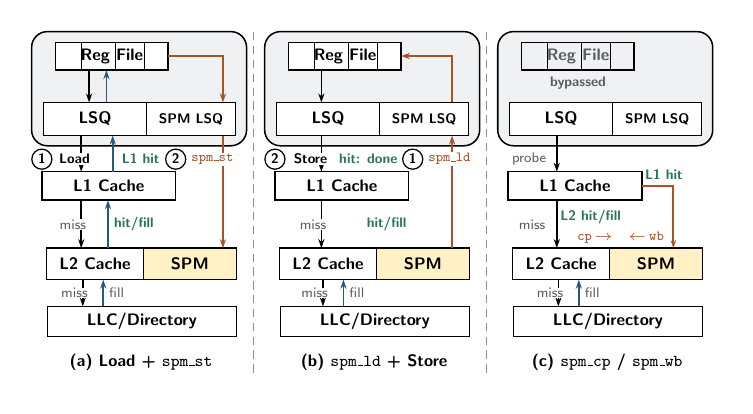
\begin{tikzpicture}[x=1cm,y=1cm]
  \path[use as bounding box] (0,0.55) rectangle (8.85,5.10);

  \skeleton{0.00}
  \skeleton{2.96}
  \skeleton{5.92}
  \draw[densely dashed, draw=separator, line width=0.48pt]
    (2.87,0.72)--(2.87,5.08);
  \draw[densely dashed, draw=separator, line width=0.48pt]
    (5.83,0.72)--(5.83,5.08);

  % -------------------------------------------------------------------------
  % (a) Two program-visible instructions: Load, then spm_st.
  \draw[request] (0.78,4.56)--(0.78,4.15);
  \draw[response] (1.00,4.15)--(1.00,4.56);
  \draw[request] (0.68,3.73)--(0.68,3.27);
  \node[circ] at (0.18,3.43) {1};
  \node[flowlabel,anchor=west] at (0.38,3.43) {Load};

  \draw[request] (0.68,2.91)--(0.68,2.30);
  \node[misslabel,anchor=west] at (0.39,2.60) {miss};
  \draw[response] (1.02,2.30)--(1.02,2.91);
  \node[hitlabel,anchor=west] at (1.08,2.60) {hit/fill};

  \draw[request] (0.70,1.90)--(0.70,1.56);
  \draw[response] (0.96,1.56)--(0.96,1.90);
  \node[misslabel,anchor=west] at (0.41,1.73) {miss};
  \node[misslabel,anchor=west] at (1.02,1.73) {fill};

  \draw[response] (1.08,3.27)--(1.08,3.73);
  \node[hitlabel,anchor=west] at (1.18,3.43) {L1 hit};

  \draw[spmpath] (1.78,4.74)--(2.48,4.74)--(2.48,4.15);
  \draw[spmpath] (2.48,3.73)--(2.48,2.30);
  \node[circ] at (1.88,3.43) {2};
  \node[flowlabel,text=bridgeorange,anchor=west]
    at (2.06,3.43) {\texttt{spm\_st}};

  \node[paneltitle] at (1.44,0.85) {(a) Load + \texttt{spm\_st}};

  % -------------------------------------------------------------------------
  % (b) Two program-visible instructions: spm_ld, then Store.
  \draw[spmpath] (5.39,2.30)--(5.39,3.73);
  \draw[spmpath] (5.39,4.15)--(5.39,4.74)--(4.74,4.74);
  \node[circ] at (4.89,3.43) {1};
  \node[flowlabel,text=bridgeorange,anchor=west]
    at (5.07,3.43) {\texttt{spm\_ld}};

  \draw[request] (3.73,4.56)--(3.73,4.15);
  \draw[request] (3.73,3.73)--(3.73,3.27);
  \node[circ] at (3.14,3.43) {2};
  \node[flowlabel,anchor=west] at (3.36,3.43) {Store};
  \node[hitlabel,anchor=west] at (3.94,3.43) {hit: done};

  \draw[request] (3.73,2.91)--(3.73,2.30);
  \node[misslabel,anchor=west] at (3.44,2.60) {miss};
  \node[hitlabel,anchor=west] at (4.29,2.60) {hit/fill};

  \draw[request] (3.75,1.90)--(3.75,1.56);
  \draw[response] (4.01,1.56)--(4.01,1.90);
  \node[misslabel,anchor=west] at (3.46,1.73) {miss};
  \node[misslabel,anchor=west] at (4.07,1.73) {fill};

  \node[paneltitle] at (4.40,0.85) {(b) \texttt{spm\_ld} + Store};

  % -------------------------------------------------------------------------
  % (c) Each labeled direction is one alternative bridge instruction.
  \draw[request] (6.72,3.73)--(6.72,3.27);
  \node[misslabel,anchor=east] at (6.60,3.43) {probe};
  \draw[request] (6.72,2.91)--(6.72,2.30);
  \node[misslabel,anchor=east] at (6.59,2.60) {miss};
  \draw[request] (6.74,1.90)--(6.74,1.56);
  \draw[response] (7.00,1.56)--(7.00,1.90);
  \node[misslabel,anchor=west] at (6.45,1.73) {miss};
  \node[misslabel,anchor=west] at (7.06,1.73) {fill};

  % The RF remains visible, but is not on the bridge data path.
  \path[box,fill=corefill] (6.27,4.56) rectangle (7.70,4.91);
  \draw[line width=0.40pt] (6.60,4.56)--(6.60,4.91);
  \draw[line width=0.40pt] (7.03,4.56)--(7.03,4.91);
  \draw[line width=0.40pt] (7.40,4.56)--(7.40,4.91);
  \node[blocklabel,text=muted] at (6.99,4.735) {Reg File};
  \node[font=\bfseries\fontsize{4.8}{5.05}\selectfont,text=muted]
    at (6.99,4.40) {bypassed};

  % spm_cp: a hit at either regular-cache level (or a lower-level fill)
  % supplies the destination SPM slot.  Hit branches are not numbered.
  \draw[directcp] (7.80,3.09)--(8.20,3.09)--(8.20,2.30);
  \node[hitlabel,anchor=south] at (8.08,3.16) {L1 hit};

  % The two arrow labels denote alternative one-instruction directions, not
  % two numbered stages. wb's coherent-store details are in Fig. 6.
  \node[hitlabel] at (7.15,2.70) {L2 hit/fill};
  \node[bridgelabel] at (7.53,2.43)
    {cp\,$\rightarrow$\quad$\leftarrow$\,wb};

  \node[paneltitle] at (7.36,0.85) {(c) \texttt{spm\_cp} / \texttt{spm\_wb}};
\end{tikzpicture}
\end{document}
